\documentclass[12pt,a4paper]{article}
\usepackage[utf8]{inputenc}
\usepackage{amsmath}
\usepackage{amssymb}
\usepackage{amsthm}
\usepackage{geometry}
\usepackage{hyperref}
\usepackage{graphicx}
\usepackage{enumerate}

\geometry{margin=1in}

\title{Strange Nested Square Roots}

\author{Nguyen Vu Hung}
\date{\today}

\begin{document}

\maketitle

\noindent Website: \url{https://vuhung16au.github.io/}\\
\noindent GitHub: \url{https://github.com/vuhung16au/}\\
\noindent LinkedIn: \url{https://www.linkedin.com/in/nguyenvuhung/}


\section{Introduction}

This document explores the fascinating properties of the discrete dynamical system defined by the recurrence relation
\[
x_{k+1} = 2x_k\sqrt{1 - x_k^2}
\]
with initial condition $x_0 \in [0,1]$. We investigate several fundamental questions:

\begin{itemize}
    \item Finding initial conditions that yield rational number sequences
    \item Identifying and characterizing the invariant measure (a probability distribution that is preserved under the transformation) of this system
    \item Establishing connections to normal numbers (numbers whose digits are uniformly distributed in every base) via the dyadic map
    \item Demonstrating ergodicity and explaining its significance
    \item Exploring connections to machine learning and artificial intelligence
\end{itemize}

The study of this system reveals deep connections between number theory, dynamical systems, ergodic theory (the mathematical study of systems where time averages equal space averages), and probabilistic methods that are fundamental to modern machine learning.

\section{The Problem}

We consider the discrete dynamical system defined by the recurrence relation:
\[
x_{k+1} = 2x_k\sqrt{1 - x_k^2}, \quad x_0 \in [0,1]
\]

The main problems of interest are:

\begin{enumerate}
    \item Find an $x_0$ such that all $x_k$ are rational numbers.
    \item Find the main \textbf{invariant measure} of this dynamical system. Explain what it means, and find related systems and their main invariant measure.
    \item Can there be more than one invariant measure?
    \item Establish the connection to \textbf{normal numbers} via the \textbf{dyadic map} (a related dynamical system).
    \item Show that these systems are \textbf{ergodic}, and explain this concept and the role that it plays.
\end{enumerate}

\subsection{Solution Outline}

Let $(p, r, q)$ be a \textbf{Pythagorean triple}, that is, $p, q, r$ are integers with $p^2 + r^2 = q^2$. If $x_k = \frac{p}{q}$, then it is easy to show that
\[
x_{k+1} = \frac{p'}{q'}
\]
with $p' = 2p\sqrt{q^2 - p^2}$, $q' = q^2$, $r' = q^2 - 2p$, defines a new Pythagorean triple $(p', q', r')$. 

So $x_0 = \frac{3}{5}$ works, answering the first question.

The invariant measure of the mapping $x \mapsto 2x\sqrt{1-x^2}$ on $[0, 1]$ is given by the probability density function:
\[
f_X(x) = \frac{2}{\pi}\frac{1}{\sqrt{1-x^2}}, \quad 0 \leq x \leq 1
\]

If you start with almost any $x_0 \in [0,1]$, the sequence $(x_k)$ is aperiodic and the \textbf{empirical distribution} of the successive values has a density approaching this invariant measure as the number of terms increases. There are exceptions: for instance, if $x_0$ is such that $x_0 = x_{10}$ (i.e., a periodic point), the sequence will not follow the main invariant measure.

Likewise, in the dyadic map $x_{k+1} = 2x_k - \lfloor 2x_k \rfloor$, if $x_0$ is a rational number, the sequence is periodic and will not follow the main invariant measure: the uniform distribution on $[0,1]$. Otherwise, $x_0$ is called a \textbf{normal number}.

The ergodic property is used in proving these results. It states that you can retrieve the invariant measure using one infinite sequence with a single seed $x_0$, or using infinitely many very short sequences $(x_0, x_1)$, each one with a random seed $x_0$.

\section{The Sequence 345}

Starting with $x_0 = \frac{3}{5}$ from the Pythagorean triple $(3, 4, 5)$, we obtain a sequence of rational numbers.

Using the recurrence relation: $x_{k+1} = 2x_k\sqrt{1 - x_k^2}$

For a Pythagorean triple $(p, r, q)$ where $p^2 + r^2 = q^2$, if $x_k = \frac{p}{q}$, then:
\[
x_{k+1} = \frac{2pr}{q^2}
\]

\subsection{Sequence Values}

Starting with $x_0 = \frac{3}{5}$ (from Pythagorean triple $(3, 4, 5)$), we obtain:

\begin{align*}
x_0 &= \frac{3}{5} \quad \text{(from Pythagorean triple $(3, 4, 5)$)} \\
x_1 &= \frac{24}{25} \quad \text{(from Pythagorean triple $(24, 7, 25)$)} \\
x_2 &= \frac{336}{625} \quad \text{(from Pythagorean triple $(336, 527, 625)$)} \\
x_3 &= \frac{354144}{390625} \quad \text{(from Pythagorean triple $(354144, 164833, 390625)$)} \\
x_4 &= \frac{116749235904}{152587890625} \quad \text{(from Pythagorean triple $(116749235904, 98248054847, 152587890625)$)}
\end{align*}

This demonstrates that the recurrence preserves the property of being a rational number when starting from a rational initial condition derived from a Pythagorean triple.

\section{The Invariant Measure}

The invariant measure of the mapping $T(x) = 2x\sqrt{1-x^2}$ on the interval $[0, 1]$ is given by the density function 
\[
p(x) = \frac{2}{\pi\sqrt{1-x^2}}
\]
with respect to the Lebesgue measure, i.e., 
\[
d\mu(x) = \frac{2}{\pi\sqrt{1-x^2}}dx
\]

\subsection{Verification Using the Perron-Frobenius Operator}

An invariant density $p(x)$ for a map $T(x)$ must satisfy the equation 
\[
p(y) = \sum_{x \in T^{-1}(y)} \frac{p(x)}{|T'(x)|}
\]
where the sum is over all preimages of $y$.

\subsubsection{Step 1: Find the Preimages}

Preimages are the values of $x$ that map to a given $y$ under the transformation $T$. In other words, they are the solutions to $T(x) = y$.

For a given $y \in (0, 1)$, the equation $y = 2x\sqrt{1-x^2}$ has two solutions for $x$, which are the preimages of $y$:
\[
x_1 = \sqrt{\frac{1+\sqrt{1-y^2}}{2}} \quad \text{and} \quad x_2 = \sqrt{\frac{1-\sqrt{1-y^2}}{2}}
\]

\subsubsection{Step 2: Calculate the Derivative}

The derivative of the map is:
\[
T'(x) = \frac{2-4x^2}{\sqrt{1-x^2}}
\]

\subsubsection{Step 3: Substitute into the Transfer Operator Equation}

If we propose the invariant density $p(x) = \frac{C}{\sqrt{1-x^2}}$ for some constant $C$, we find that for the two preimages $x_1$ and $x_2$, the sum is:
\[
\frac{p(x_1)}{|T'(x_1)|} + \frac{p(x_2)}{|T'(x_2)|} = \frac{C}{2\sqrt{1-y^2}} + \frac{C}{2\sqrt{1-y^2}} = \frac{C}{\sqrt{1-y^2}}
\]

The result of the sum is exactly the form of the proposed density, $p(y)$, which confirms that it is an invariant density.

\subsubsection{Step 4: Normalize the Density}

To be a valid probability measure, the integral of the density over the domain $[0, 1]$ must equal 1:
\[
\int_0^1 \frac{C}{\sqrt{1-x^2}}dx = C[\arcsin(x)]_0^1 = C(\arcsin(1)-\arcsin(0)) = C(\pi/2 - 0) = \frac{C\pi}{2}
\]

Setting this equal to 1 gives $C = \frac{2}{\pi}$.

Therefore, the invariant density is 
\[
p(x) = \frac{2}{\pi\sqrt{1-x^2}}
\]

This map is a specific case of a family of maps known as \textbf{Chebyshev maps} (dynamical systems defined by Chebyshev polynomials, which are a family of orthogonal polynomials defined recursively as $T_n(\cos\theta) = \cos(n\theta)$ and which appear as trigonometric polynomial maps that exhibit chaotic behavior), for which this measure is a well-known result.

\subsection{Numerical Verification}

To verify the theoretical result, we numerically simulate the sequence starting from an initial condition $x_0 = \frac{3}{4}$ and compute the empirical density. The simulation generates 100,000 iterations using the recurrence relation $x_{k+1} = 2x_k\sqrt{1-x_k^2}$, and the empirical distribution of the values is computed using a histogram.

\begin{figure}[htbp]
\centering
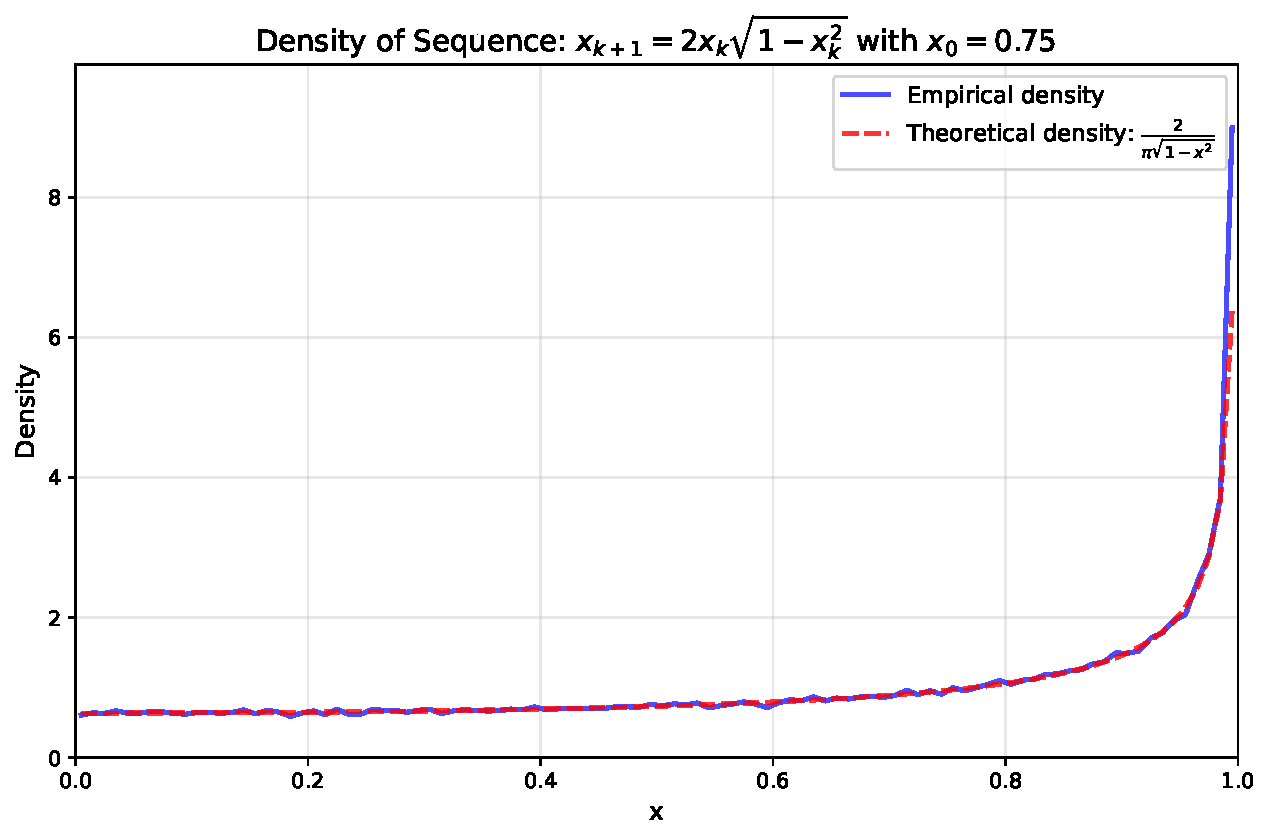
\includegraphics[width=0.8\textwidth]{data/density_0.75.pdf}
\caption{Empirical density of the sequence $x_{k+1} = 2x_k\sqrt{1-x_k^2}$ with initial condition $x_0 = \frac{3}{4}$, compared with the theoretical invariant density $p(x) = \frac{2}{\pi\sqrt{1-x^2}}$. The simulation shows excellent agreement between the empirical distribution (blue line) and the theoretical prediction (red dashed line), confirming that the invariant measure is indeed given by the stated formula.}
\label{fig:density}
\end{figure}

Figure~\ref{fig:density} shows the empirical density obtained from the simulation alongside the theoretical invariant density. The excellent agreement between the two demonstrates that for typical initial conditions, the long-term empirical distribution of the sequence converges to the theoretical invariant measure, as predicted by ergodic theory.

\section{The Dyadic Map}

A dyadic map is a simple but important mathematical function in chaos theory and dynamical systems. It's defined as 
\[
f(x) = 2x - \lfloor 2x \rfloor
\]
where $\lfloor 2x \rfloor$ is the floor function, which gives the greatest integer less than or equal to $2x$. The map is also called the \textbf{2x mod 1} map because it is equivalent to $f(x) = 2x \pmod{1}$. This map takes any number in the interval $[0, 1)$ and stretches it by a factor of two, then takes the fractional part, effectively folding the interval back onto itself.

The name ``dyadic'' refers to \textbf{base-2} or binary numbers. The dyadic map is closely linked to the binary representation of a number. If a number $x$ is represented in binary as $0.b_1b_2b_3...$, applying the dyadic map, $f(x)$, is equivalent to a \textbf{left shift} of the binary digits. For example, if $x = 0.10110...$ in binary, then $2x = 1.0110...$, and $f(x) = 0.0110...$. The first digit, $b_1$, is ``shifted'' to the left of the decimal point and removed, and the rest of the digits follow.

\subsection{Dyadic Map and Normal Numbers}

The dyadic map provides a clear connection to the concept of \textbf{normal numbers}. A number is \textbf{normal} in base 2 if, in its binary representation, every finite sequence of digits appears with the same limiting frequency as every other sequence of the same length. The dyadic map helps prove that for almost all initial values $x_0 \in [0, 1)$, the sequence generated by iterating the map, $(x_k)$, has a \textbf{uniform distribution}. This means that over a long period, the values of $x_k$ will be evenly distributed across the interval $[0, 1)$.

\begin{itemize}
    \item If $x_0$ is a \textbf{rational number} 
    its binary expansion is either terminating or repeating. Iterating the dyadic map on a rational number leads to a \textbf{periodic sequence} of values, meaning it will eventually repeat itself. For example, starting with $x_0 = 1/3 = 0.010101..._2$ leads to the sequence $1/3, 2/3, 1/3, 2/3, ...$ which does not uniformly fill the interval.
    \item If $x_0$ is an \textbf{irrational number}, the sequence of values will not repeat. For most irrational numbers, the empirical distribution of the sequence $(x_k)$ will approach the uniform distribution on $[0,1]$. A number is normal in base 2 if and only if the sequence of its dyadic map iterations is uniformly distributed. This is a powerful result, connecting a property of a number's digits to the behavior of a dynamical system.
\end{itemize}

The \textbf{main invariant measure} for the dyadic map is the \textbf{uniform distribution on $[0, 1)$}. This is the distribution that is preserved by the map. If you take a collection of points distributed uniformly and apply the dyadic map, the new collection of points will also be uniformly distributed.

\subsection{Ergodicity of the Dyadic Map}

The dyadic map is an \textbf{ergodic system} (a dynamical system where time averages equal space averages, meaning a single trajectory's long-term behavior reflects the statistical properties of the entire system). In simple terms, ergodicity means that the long-term time average of a single trajectory of the system is the same as the average over all possible starting points at a single moment in time.

For the dyadic map, this means:

\begin{enumerate}
    \item \textbf{Time average:} If you take a single initial value $x_0$ (as long as it's not a rational number) and iterate the dyadic map to generate a long sequence $(x_0, x_1, x_2, ...)$, the average behavior of this single sequence will statistically reflect the entire system. For instance, the frequency of values falling into any subinterval of $[0, 1)$ will be proportional to the length of that subinterval.
    \item \textbf{Ensemble average:} The average over all possible initial values in $[0, 1)$ at a given time is also a uniform distribution.
\end{enumerate}

The ergodicity of the dyadic map allows us to study the behavior of a typical infinite sequence starting from a single number and draw conclusions about the properties of almost all numbers. For example, it helps to prove that almost all numbers are normal, even though we can't explicitly construct many of them.

More than one invariant measure can exist. For the dyadic map, the uniform distribution is the \textbf{main} or \textbf{unique absolutely continuous invariant measure} (a measure that has a probability density function). However, there are also other invariant measures, such as \textbf{discrete invariant measures}. For instance, a measure that assigns probability 1 to a single fixed point (e.g., $x=0$) is an invariant measure. If the system is \textbf{ergodic}, it means that any invariant measure can be decomposed into a sum of ergodic measures.

\section{The Ergodic Theorem}

The \textbf{Ergodic Theorem} is one of the most fundamental results in dynamical systems theory and statistical mechanics. It provides a bridge between the microscopic behavior of individual trajectories and the macroscopic statistical properties of a system.

\subsection{Mathematical Formulation: Birkhoff's Ergodic Theorem}

\textbf{Theorem (Birkhoff, 1931):} Let $(X, \mathcal{B}, \mu, T)$ be a measure-preserving dynamical system, where:
\begin{itemize}
    \item $X$ is a measurable space
    \item $\mathcal{B}$ is a $\sigma$-algebra
    \item $\mu$ is a probability measure
    \item $T: X \to X$ is a measure-preserving transformation
\end{itemize}

For any integrable function $f: X \to \mathbb{R}$ (i.e., $\int |f| d\mu < \infty$), the \textbf{time average}
\[
\lim_{n \to \infty} \frac{1}{n} \sum_{k=0}^{n-1} f(T^k(x))
\]
exists for $\mu$-almost every $x \in X$.

If the system is \textbf{ergodic}, then this time average equals the \textbf{space average}:
\[
\lim_{n \to \infty} \frac{1}{n} \sum_{k=0}^{n-1} f(T^k(x)) = \int_X f \, d\mu
\]
for $\mu$-almost every $x \in X$.

\subsection{Intuitive Explanation}

The Ergodic Theorem tells us that in well-behaved dynamical systems:

\begin{enumerate}
    \item \textbf{Time Average = Space Average:} The long-term behavior of a single trajectory mirrors the overall statistical behavior of the entire system.
    \item \textbf{Individual vs. Ensemble:} Instead of studying the entire ensemble of possible states, we can understand the system's properties by following one typical trajectory for a long time.
    \item \textbf{Statistical Regularity:} Even though individual trajectories may appear chaotic or unpredictable, their long-term statistical properties are deterministic and predictable.
\end{enumerate}

\subsection{Key Concepts}

\subsubsection{Measure-Preserving Transformation}
A transformation $T$ is \textbf{measure-preserving} if $\mu(T^{-1}(A)) = \mu(A)$ for all measurable sets $A$. This means the transformation preserves the ``volume'' or ``probability'' of regions.

\subsubsection{Ergodicity}
A measure-preserving system is \textbf{ergodic} if it cannot be decomposed into smaller invariant components. Mathematically, if $T^{-1}(A) = A$ implies $\mu(A) = 0$ or $\mu(A) = 1$.

Intuitively, ergodicity means:
\begin{itemize}
    \item The system is ``irreducible'' --- you can't break it into disconnected parts
    \item Trajectories are ``mixing'' --- they eventually visit all regions of the space
    \item The system has no non-trivial conserved quantities
\end{itemize}

\subsection{The Dyadic Map and Normal Numbers}

The \textbf{dyadic map} provides an elegant and powerful framework from dynamical systems theory to establish the existence of \textbf{normal numbers}. The connection is a direct consequence of the \textbf{Ergodic Theorem}.

If we write a number $x$ in binary as $x = 0.b_1b_2b_3...$, where each $b_i$ is a 0 or a 1, then applying the map $T$ to $x$ simply shifts its binary digits one position to the left, dropping the first digit.

By applying the Ergodic Theorem, we can connect time averages to space averages:
\[
\text{Time Average} = \lim_{N \to \infty} \frac{1}{N} \sum_{n=0}^{N-1} f(T^n(x)) = \int_0^1 f(x) \,dx = \text{Space Average}
\]

The time average represents the frequency of a digit (or block of digits) in the binary expansion of $x$. The space average represents the expected probability of that digit (or block) in a uniform distribution.

The theorem guarantees that for ``almost all'' numbers (meaning all numbers except for a set of measure zero, like the rationals), the frequency of any binary digit (0 or 1) will be exactly $1/2$. This can be extended to show that the frequency of any block of binary digits of length $k$ will be exactly $1/2^k$. This is precisely the definition of a \textbf{binary normal number}.

\section{Conclusion: Connections to Machine Learning and AI}

The study of dynamical systems, invariant measures, and ergodic theory has profound implications for machine learning and artificial intelligence. These connections manifest in several key areas:

\subsection{Sampling and Monte Carlo Methods}

The ergodic property --- that time averages equal space averages --- is fundamental to \textbf{Monte Carlo methods}, which are ubiquitous in machine learning. When we use Markov Chain Monte Carlo (MCMC) methods to sample from complex probability distributions, we rely on the ergodic properties of the Markov chain to ensure that the long-term behavior of a single trajectory accurately represents the target distribution. This is exactly what the Ergodic Theorem guarantees: by following one trajectory for a sufficiently long time, we can recover the invariant measure.

\subsection{Normalization and Representation Learning}

The connection between normal numbers and the dyadic map reveals fundamental properties about how numbers are represented in different bases. In machine learning, we often work with numerical representations in various forms (binary, decimal, floating-point, etc.). Understanding the ergodic properties of these representations helps us design better normalization schemes and understand the statistical properties of data transformations.

\subsection{Invariant Representations}

The concept of an \textbf{invariant measure} is directly related to learning \textbf{invariant representations} in deep learning. Just as the dynamical system preserves its invariant measure under transformation, neural networks often seek to learn representations that are invariant to certain transformations (e.g., translation, rotation, scaling). The mathematical framework of invariant measures provides a theoretical foundation for understanding why and how such representations can be learned.

\subsection{Stochastic Processes and Neural Networks}

Recurrent neural networks (RNNs) and their variants can be viewed as discrete dynamical systems. Understanding the ergodic properties and invariant measures of such systems helps us:

\begin{itemize}
    \item Analyze the long-term behavior of RNNs
    \item Design stable architectures that avoid vanishing or exploding gradients
    \item Understand how networks preserve or forget information over time
\end{itemize}

\subsection{Generative Models}

Generative models, such as Variational Autoencoders (VAEs) and Generative Adversarial Networks (GANs), learn to approximate probability distributions. The theory of invariant measures provides insights into:

\begin{itemize}
    \item How generators learn to produce samples from target distributions
    \item The convergence properties of training algorithms
    \item Why certain architectures or training procedures lead to stable distributions
\end{itemize}

\subsection{Theoretical Guarantees}

The mathematical rigor of ergodic theory provides \textbf{theoretical guarantees} about the behavior of learning algorithms. Just as the Ergodic Theorem guarantees that time averages converge to space averages for ergodic systems, we can prove convergence guarantees for machine learning algorithms that rely on iterative updates and sampling.

\subsection{Future Directions}

The deep connections between ergodic theory and machine learning suggest several promising research directions:

\begin{itemize}
    \item Using ergodic theory to analyze and improve optimization algorithms
    \item Applying invariant measure concepts to understand generalization in deep learning
    \item Developing new sampling methods based on ergodic properties of neural network dynamics
    \item Using dynamical systems theory to design more stable and efficient architectures
\end{itemize}

In conclusion, the strange nested square roots system and its associated mathematical framework of invariant measures, ergodic theory, and normal numbers form a rich theoretical foundation that underlies many practical techniques in modern machine learning and artificial intelligence. Understanding these connections not only deepens our theoretical understanding but also provides guidance for developing more effective and theoretically grounded learning algorithms.

\end{document}

